\subsection{\mu Slave Module (\mu S)}

\mu S is a microcontroller that receives measurement data via the I2C bus and uploads this data to a public mqtt broker via
GSM (GPRS).

\subsubsection{Requirements}
Originally, I planed to use only the  \cite{noauthor_arduino_2020} DK to realize the entire application.
It turned out however, that I was unable to put the u-blox GSM module hosted on the DK into low power mode.
While I was able to obtain some power consumption reduction via the Arduino GSM library, this was by far not enough
for a low power application. I decided therefore to split the functionality across two DKs: one who does the actuals water
flow measurement - the master -  and another separate GSM enabled module - the slave -
to perform actual data transmission.
The master would then control the slave power supply such that the slave and the radio module would only draw current
during the relatively short period required for data transmission.
Hence, the requirements for \mu S are:

\begin{enumerate}
    \item bidirectional data flow between master and slave.
    \item GSM/GPRS compatible modem.
\end{enumerate}

The \cite{noauthor_arduino_2020} provides an I2C interface and fulfills both requirements.
Another solution would have been to simply find a UART-compatible radio module (without additional microcontroller).
While this would have resulted in a simpler and more compact circuit, I would have had to adapt the Arduino GSM library or write
one from scratch.

\subsubsection{Implementation}
\begin{table}[H]
    \centering
    \begin{tabularx}{\linewidth}{>{\hsize=0.25\hsize}X
            >{\hsize=1\hsize}X >{\hsize=1\hsize}X
            >{\hsize=0.5\hsize}X >{\hsize=2.25\hsize}X}
        Id    & BOM Item                     & Order Code & Package  & Rationale                 \\
        \midrule
        $U_1$ & \cite{noauthor_arduino_2020} &            & DIL (28) & availability, ease of use \\
    \end{tabularx}
    \caption{\mu S - BOM}
\end{table}
\begin{table}[H]
    \centering
    \begin{threeparttable}[b]
        \begin{tabularx}{\linewidth}{ >{\hsize=.15\hsize}X >{\hsize=1.35\hsize}X >{\hsize=1.5\hsize}X }
            Id & Issue                               & Potential solution                          \\
            \midrule
            1  & $U_1$: GMS 3 only, chipset obsolete & select a GSM LTE or LTE-M generation module \\
        \end{tabularx}
    \end{threeparttable}
    \caption{\mu S - Issues}
\end{table}

\clearpage
\begin{figure}[h]
    \centering
    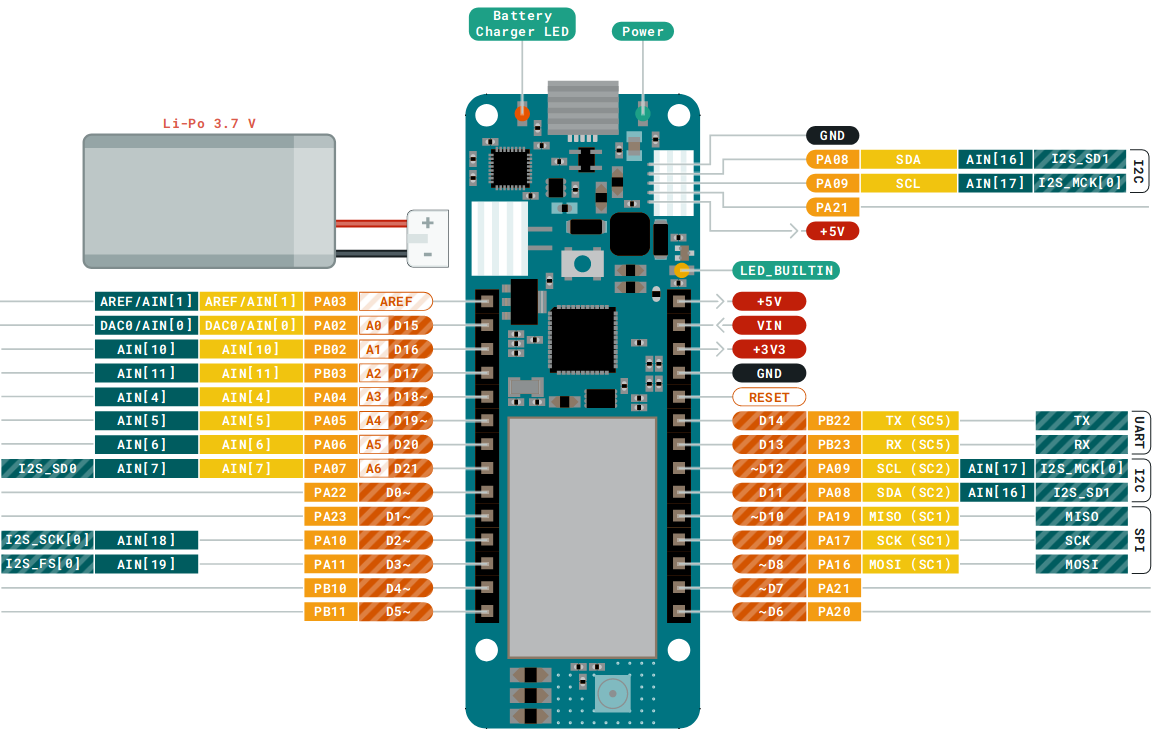
\includegraphics[width=1\textwidth]{SL/uS/uS}
    \caption{\mu S - pin out \cite{noauthor_arduino_2020}}
\end{figure}
\begin{table}[H]
    \centering
    \begin{threeparttable}[b]
        \begin{tabularx}{\linewidth}{ >
                    {\hsize=.25\hsize}X >
                    {\hsize=0.5\hsize}X >
                    {\hsize=.25\hsize}X  >
                    {\hsize=.5\hsize}X >
                    {\hsize=.25\hsize}X  >
                    {\hsize=3\hsize}X
            }
                  & \multicolumn{4}{c}{Pin mapping} &                                                                                                            \\
            \cmidrule(lr){3-6}
            Id    & Net                             & Nb. & Name           & Type               & Function                                                       \\
            \midrule
            $U_1$ & .CON                            & 9   & \texttt{A0}    & \rightharpoonup    & high: connect I2C bus to master (bypass the isolation barrier) \\
            $U_1$ & .ACK                            & 10  & \texttt{D0}    & \rightharpoonup    & high: signal to master that I am ready to receive data         \\
            $U_1$ & .CS                             & 11  & \texttt{D1}    & \rightharpoonup    &                                                                \\
            $U_1$ & EWD                             & 12  & \texttt{D5}    & \rightharpoonup    & enable WD                                                      \\
            $U_1$ & RWD                             & 13  & \texttt{D5}    & \rightharpoonup    & reset WD                                                       \\
            $U_1$ & .MISO                           & 17  & \texttt{D2}    & \leftharpoonup     &                                                                \\
            $U_1$ & .SCK                            & 18  & \texttt{D3}    & \rightharpoonup    &                                                                \\
            $U_1$ & .MOSI                           & 19  & \texttt{D4}    & \rightharpoonup    &                                                                \\
            $U_1$ & .SDA                            & 20  & \texttt{SDA}   & \leftrightharpoons &                                                                \\
            $U_1$ & .SCL                            & 21  & \texttt{SCL}   & \rightharpoonup    &                                                                \\
            $U_1$ & \neg RS                         & 24  & \texttt{RESET} & \leftharpoonup     & pulled down by WD timer or user button in case of timeout      \\
            $U_1$ & \Gnd                            & 25  & \texttt{GND}   & \Gnd               &                                                                \\
            $U_1$ & .3V3                            & 26  & \texttt{VCC}   & $\rightarrow$      & regulated output voltage\tnote{1}                              \\
            $U_1$ & .V\textsubscript{\mu S}         & 27  & \texttt{VIN}   & $\leftarrow$       & input voltage controlled by \mu M                              \\
        \end{tabularx}
    \end{threeparttable}
\end{table}
\clearpage
